\section{実験方法}

\subsection{試験片の作製}

\begin{enumerate}
    \item ポリプロピレン(サンアロマー PM600A)のペレットをおよそ11.2g-11.5g用意し,ステンレス板の上に置いた型枠に入れた.この際,気泡が生じないようにできる限りペレットを敷き詰めた.
    \item 型枠の上に別のステンレス板を置き,熱プレス機の下部ヒータの上に設置した.
    \item 上のステンレス板が上部ヒータに触れるまで下部ヒータを上げ,そのまま1分程度保持した.ペレットが解け始めたらゆっくりと15MPaまで圧力をかけてそのまま3分待機した.
    \item 型枠ごと2枚のステンレス板をクランプで挟み,すぐに水中に入れて急冷した.
    \item 2枚目の板材は1-4の手順を同様に行い,さらに型枠ごと2枚のステンレス板を65$^\circ$Cに設定された別の熱プレス機で10分間15MPaで保持した.その後水冷した.
    \item 3枚目は保持する温度を120$^\circ$Cに設定して作成した.
    \item 作成した板材に打ち抜き加工を実施し,ISO37-3試験片の形に成形した(図\ref{fig:試験片}).
    \item 試験片に対して
    \item 標線とつかみ部を示すマーキングを施した(図\ref{fig:試験片}赤線).
    \item 標線間距離および平滑部の幅・厚さをノギス・マイクロメータで測定した.
\end{enumerate}

\begin{figure}[htbp]
    \centering %中央揃え
    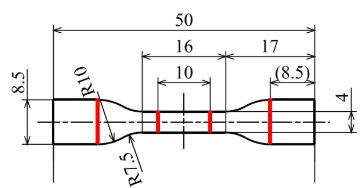
\includegraphics[width=100truemm,clip]{fig/fig_試験片.png}
    \caption{ISO37-3 Specimen Shape.}
    \label{fig:試験片}
\end{figure}

\subsection{単軸引張試験}

\begin{enumerate}
    \item 引張試験機の「ZERO」ボタンを長押しして「LOAD」の表示を「0.00」にした.
    \item 試験片を引張試験機の上部治具,下部治具の順に設置した.
    \item カメラの位置で画角を調整し,レンズ部分のつまみで最適なピント・明るさに設定した.
    \item カメラの直線検出範囲を画像認識システムコントローラで設定した.
    \item 制御用PCのデスクトップにある「ストログラフ」アイコンから「ストログラフデータ処理」を起動して環境設定を行った(ロードセル容量1,000N,試験速度5mm/min).
    \item 制御用PCのソフト上で試料設定項目の入力(試験本数,試料サイズ)を行った.
    \item 制御用PCのソフトから「たるみとり」を実行し,引張試験機の「ZERO」ボタンを押して「STROKE」を「0.00」にした.
    \item 制御用PCの「GL-connection」(起動済み)で記録を開始し,即座に「ストログラフデータ処理」で試験を開始した.
    \item 試験終了後すぐに「GL-connection」で記録を停止した.
\end{enumerate}

\subsection{材料組織観察}

\begin{enumerate}
    \item 作製した板材をミクロトームで薄片化してスライドガラスに挟んだ.
    \item 透過偏光顕微鏡を用いて材料組織の観察を行った.
\end{enumerate}